\section{Chart::Points}
\herv{Name:} Chart::Points\\ \\
\herv{File:} Points.pm\\ \\
\herv{Requires:}Chart::Base, GD, Carp, FileHandle\\ \\
\herv{Description:} \fett{Points} is a \fett{subclass} of Chart::Base.\\
The class Points creates a point chart.\\
\\
\herv{Example:}
\begin{figure}[h]
	\begin{center}
		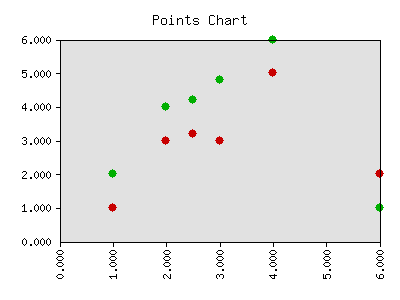
\includegraphics[scale=0.5]{points.png}
	\end{center}
	\caption{Points chart}
	\label{fig:points}
\end{figure}
\begin{verbatim}
use Chart::Points;

$g = Chart::Points->new();
$g->add_dataset (1, 4,   3, 6, 2, 2.5);  # x-coordinates
$g->add_dataset (1, 5,   3, 2, 3, 3.2);  # y-coordinates dataset 1
$g->add_dataset (2, 6, 4.8, 1, 4, 4.2);  # y-coordinates dataset 2

@hash = ('title' => 'Points Chart',
         'xy_plot' => 'true',
         'x_ticks' => 'vertical',
         'legend' => 'none',
         'sort' => 'true',
         'precision' => 3,
         'include_zero' => 'true',
	 );

$g->set (@hash);

$g->png ("Grafiken/points.png");

\end{verbatim}
\herv{Constructor:} An instance of a points chart object can be created with the constructor new():\\
\fett{\$obj = Chart::Points->new();}\\
\fett{\$obj = Chart::Points->new(\kursiv{width}, \kursiv{height});}\\
\\
If \fett{new} has no arguments, the constructor returns an image with the size 300x400 pixels. If new has two arguments \kursiv{width} and \kursiv{height}, it returns an image with the desired size. \\ 
\\ 
\herv{Methods:}All universally valid methods, see page \pageref{methods}: Chart::Base. \\
\\
\herv{Attributes/Options:} All universally valid options, see page \pageref{options}. Also available these special options:
\begin{description}
\item['y\_axes'] Tells chart where to place the y-axis. Valid values are 'left', 'right' and 'both'. Defaults to 'left'.
\item['pt\_size']Sets the radius of the points in pixels. Default is 18.
\item['sort']Sorts the data of a x-y-graph ascending if set to 'true'. Should be set if the added data isn't sorted. Defaults to 'false'.
\item['xy\_plot']Forces Chart to plot a x-y-graph, which means that the x-axis is also numeric if set to 'true'. Very useful for plots of mathematical functions. Defaults to 'false'.
\end{description}